\documentclass[12pt]{article}

\usepackage{mathtools} 
\usepackage{cite}
\usepackage{graphicx}
\usepackage{listings}
\usepackage{wrapfig}

\title{Introduction to hypergraphs and odometers}
\author{
        Roscoe Casita \\
        CIS 503: Thesis\\
}
\date{\today}


\begin{document}
\maketitle

\begin{abstract}
Hypergraph implementations have modeled real life systems with material gains in performance over graph representations of the same problems. Odometers serve as an alternative representation of hyperedges in a hypergraph from the traditional incident matrix. The traversal of hyperedges in a hypergraph using an odometer and incrementing function is shown to be similar to traversing a Hilbert curve through a $N^\infty$ dimensional Hilbert space.
\end{abstract}

\section{Introduction}
Hypergraphs are composed of a set of vertexes and hyperedges $HG = (v, he)$ commonly denoted in matrix format show below. Each column represents a node’s set of hyperedges. Each row represents a set of nodes in a hyperedge. The sample hypergraph presented as both nodes linked by hyperedges and hyperedges linked by nodes in the subsequent pictures. Displaying high dimensionality objects such as hypergraphs is a complex problem with active ongoing research in the area..
\begin{center}
\begin{tabular}{l | c | r}

\begin{tabular}{l l l l l l l l}
			 & $V_1$ & $V_2$ & $V_3$ & $V_4$ & $V_5$ & $V_6$ \\
$E_1$  &     1 		& 1          & 1 			& 0 			& 0 			& 0 		 \\
$E_2$  &     0 		& 1          & 1 			& 0 			& 0 			& 0 		 \\
$E_3$  &     0 		& 0          & 1 			& 0 			& 1 			& 1 		 \\
$E_4$  &     0 		& 0          & 1 			& 1			& 0 			& 0 		 \\
$E_5$  &     1 		& 0          & 0 			& 1			& 0 			& 1 		 \\
\end{tabular}

& 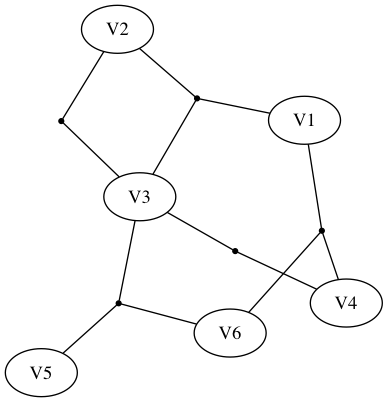
\includegraphics[scale=.20]{vertex_graph} & 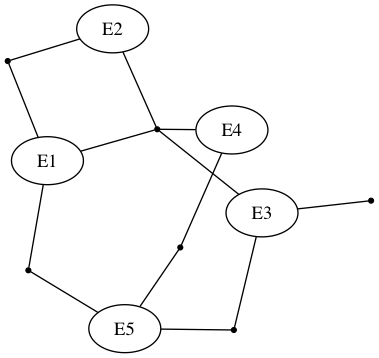
\includegraphics[scale=.20]{edge_graph}\
\end{tabular}
\end{center}


\newpage

\section{Hypergraph, odometer \& hyperedge:}
An ordered vector is a mapping of numbers to addresses in an array of things. Thus a number can be used to retrieve and set a value at that numeric address. A hypergraph is an ordered vector of type $T$ nodes and a mapping of type $T$ node values to numbers. Access time for arrays is $O(c)$. In both get functions the access time is $O(n)$ where $n$ is the magnitude of the edge/odometer. As all objects are vector arrays, these loops can all potentially be executed in parallel changing the runtime to $O(n/p)$ where $p$ is the number of processors able to execute the address lookup.
\begin{lstlisting}
def makeHyperGraph(hyperedge):
    vector_things = [0 for x in range(len(hyperedge))]
    address_lookup = dict()
    for i in range(len(hyperedge)):
        node = hyperedge[i]
        vector_things[i] = node
        address_lookup[node] = i
    return (vector_things,address_lookup)

def getHyperEdge(hypernet,odometer):
    (vector_things,address_lookup) = hypernet
    hyperedge = [0 for x in range(len(odometer))]
    space_size = len(vector_things)
    for index in range(len(odometer)):
        node_index = odometer[index] % space_size
        hyperedge[index] = vector_things[node_index]
    return hyperedge
    
def getOdometer(hypergraph,hyperedge):
    (vector_things,address_lookup) = hypergraph
    odometer = [0 for x in range(len(hyperedge))]
    for index in range(len(hyperedge)):
        node = hyperedge[index]
        odometer[index] = address_lookup[node]
    return odometer
\end{lstlisting}
\newpage
\begin{wrapfigure}{r}{0.5\textwidth}
  \begin{center}
    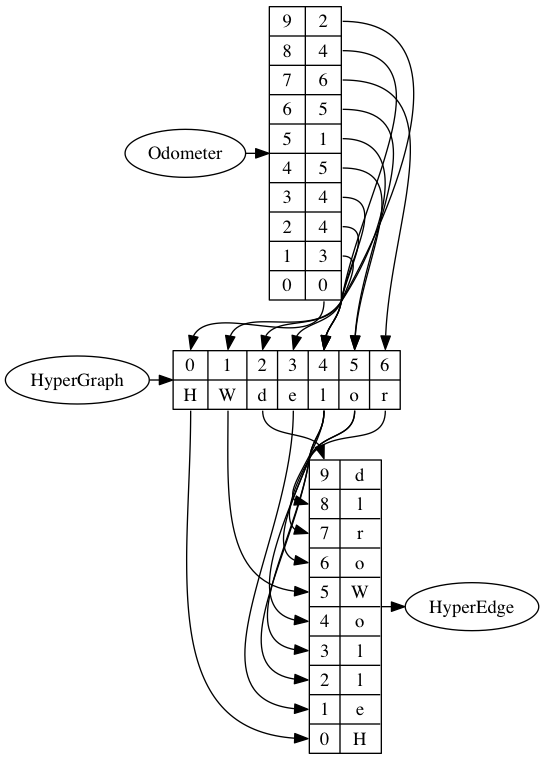
\includegraphics[width=0.48\textwidth]{odometers}
  \end{center}
\end{wrapfigure}

\section{Concepts}

\indent The presented hypergraph model supports conversion from an odometer to hyperedge or hyperedge to odometer in one function call. Traditionally all hyperedges in a hypergraph are explicitly declared and stored in memory or disk. \\

This model can explore super dense hypergraphs: $2^N$, $N^N$ even $N^M$ hyperedges that standard matrix hypergraph models cannot represent. These hypergraphs share the common characteristic that they must be explored algorithmically. This image demonstrates a single odometer to hyperedge conversion via arbitrary hypergraph using the given definitions.\\

\begin{lstlisting}
hypergraph =makeHyperGraph(sorted(set("Hello World!")))

odometer = getOdometer(hypergraph, "Hello World!")

hyperedge = getHyperEdge(hypergraph,odometer)

(vector_of_things,address_lookup) = hypergraph
\end{lstlisting}

\newpage
\section{To Do:}\label{results}

\begin{itemize}
	\item Demonstrate how a hypergraph is an underlying data structure that is not well standardized. Show how hypergraphs can be adapted with odometers over runtime to emulate lists, queues, stacks, possibly / talk about how an odometer corresponding to the correct sort order of a hypergraph is unique to that hypergraph.
	\item Code \& draw fully connected graph (simple, terminates), all paths through a graph (complex, runs incrementally forever), tree dfs/bfs odometer (complex, terminates),  draw fringe of a reaction forest of trees (complex, unknown termination).
	\item Show howoOdometers allow a program to change  position in as many steps as it takes to set the numbers in the odometer. $O(n)$ to set the odometer and $O(n)$ to access the hyperedge results in a total time of $O(n+n) \rightarrow O(2n) \rightarrow O(n)$ to traverse from any hyperedge to any hyperedge.
	\item Visiting all hyperedges is impossible. There domain of each number in an odometer is from $\{-\infty,+\infty\}$ and there are $N$ numbers in an odometer so there are $\infty^N$ configurations of a single odometer of size $N$. Thus there are an infinite amount of hyperedges for all hypergraphs that this system represents. 
	\item Odometer state + function define the Hilbert space and Hilbert curve through that space simultaneously. A set of odometers with the same number only reference the same node if they are associate with the a single unique hypergraph.
	\item The odometer allow indexing negatively (reverse indexing of a list) and modulo rounding (index past the end of the array results in starting again at the beginning of the array). This function is not reversible as the mapping is from $\{-\infty,\infty\}^m \rightarrow \{0,N\}^m$, where $m$ is the number of numbers in the odometer...
	\item Thus all odometers are valid for any hypergraph, but not all hyperedges are valid for any hypergraph. They would be valid if the set of nodes contained in the hyperedge is also contained in the hypergraph. (This might be a lead in for Godel's work with number mapping systems, and recent information on category theory in mathematics.)
	\item The reaction project uses a custom odometer incremental function that treats the search space as a forest of trees, traversing each tree until a mass balanced equation is found from the set of compounds along the pathway to the node. This becomes the fringe of the search tree which is collected as the hypergraph of interest. 
	
\end{itemize}
\section{Questions}
\begin{itemize}
\item Dr. Hank Childs talked about primitives in parallel processing language, what are the primitives and how are they used? What algorithms can be written using them?
\item What library $should$ be used to write distributed code? CUDA, OpenACC, OpenCL, NET Parallel, Thrust, etc? Distributed system here at University of Oregon? 
\item 
\end{itemize}
\bibliographystyle{abbrv}
\bibliography{Introduction}

\end{document}